\documentclass{standalone}
\usepackage{tikz}
\usetikzlibrary{patterns, angles}

\begin{document}
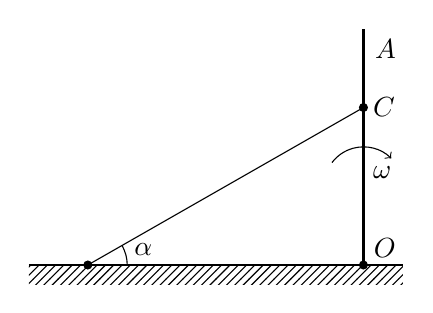
\begin{tikzpicture}
	\coordinate (O) at (4, 0);
    \coordinate (C) at (4, 2);
    \coordinate (A) at (4, 3);
    \coordinate (D) at (4.5, 0);
    \coordinate (B) at (0.5, 0);
    \coordinate (M1) at (0, 4);
    \coordinate (M2) at (7, 4);
    \coordinate (M3) at (4, 1);    
       
	\draw [draw=none, pattern=north east lines] (D) rectangle (-0.25,-0.25);
	\draw [thick] (O) node [above=6pt, right] {$O$} -- (A) node [right=8pt, below] {$A$};
	\draw [thick] (-0.25,0) -- (D);		
	\draw [fill] (C) circle (0.05);	
	\draw [fill] (B) circle (0.05);
	\draw [fill] (O) circle (0.05);
	\draw (B) -- (C) node [right] {$C$};
	\pic [draw, -, angle eccentricity=1.5] {angle = O--B--C};
	\node [right=20pt, above] at (B) {$\alpha$};
	\pic [draw, <-, angle eccentricity=1.5] {angle = M2--M3--M1};
	\node [above=5pt, right] at (M3) {$\omega$};
\end{tikzpicture}
\end{document}